\chapter{Condiciones del problema.}\label{sec:Condiciones del problema.}
\setcounter{figure}{0}
\setcounter{equation}{0}
La situación en la que nos enfrentamos en el problema es de una onda electromagnetica incidente en nuestro microhilo. Esta onda tiene un campo magnético incidente $B_i$ y un campo eléctrico incidente $E_i$. Denominaremos al volumen del micro-hilo como $\Omega_1$ y al volumen externo como $\Omega_2$ tal como se muestra en la figura \ref{fig:Representacion del problema}.
\begin{figure}[H]
\centering
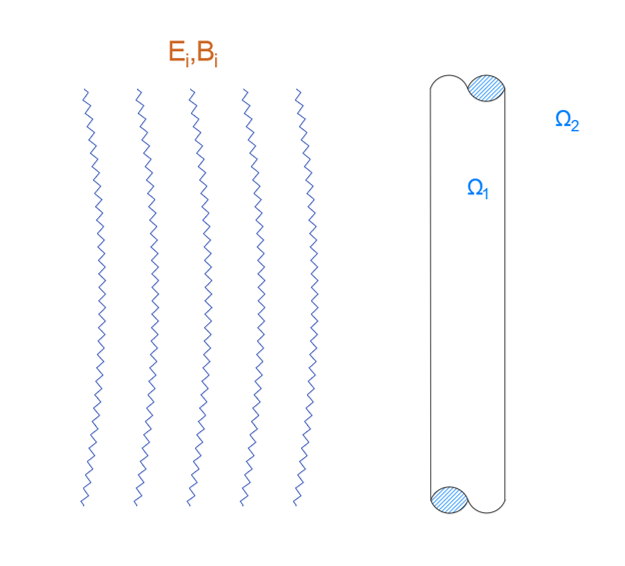
\includegraphics[width=8cm]{Imagenes/ondaincidente.png}
\caption{Situación del problema} \label{fig:Representacion del problema}
\end{figure}
Comenzaremos con las ecuaciones de Maxwell:
\begin{equation}
\begin{split}
&\nabla\cdot\textbf{D} = \rho\qquad\nabla\times\textbf{E} = -\frac{\partial\textbf{B}}{\partial t}\\
&\nabla\cdot\textbf{B} = 0\qquad\nabla\times\textbf{H} = J_f+\frac{\partial\textbf{D}}{\partial t}
\end{split}
\label{eq: Maxwell_inicial}
\end{equation}
Reescribiendo la ecuación \eqref{eq: Maxwell_inicial} en función solo de $B$ y $D$:
\begin{equation}
\begin{split}
&\nabla\cdot\textbf{D} = \rho\qquad \nabla\times\textbf{D} = -\varepsilon\frac{\partial\textbf{B}}{\partial t}\\
&\nabla\cdot\textbf{B} = 0\qquad\nabla\times\textbf{B} = \mu J_f+\mu\frac{\partial\textbf{D}}{\partial t}
\end{split}
\label{eq: Maxwell_soloBD}
\end{equation}
Podemos suponer que una onda incidente en un entorno con propiedades electromagnéticas $\mu_2$ y $\varepsilon_2$ sufrirá de una perturbación si se encuentra con algún objeto con propiedades diferentes, tal como se plantea en nuestro problema.
\begin{figure}[H]
\centering
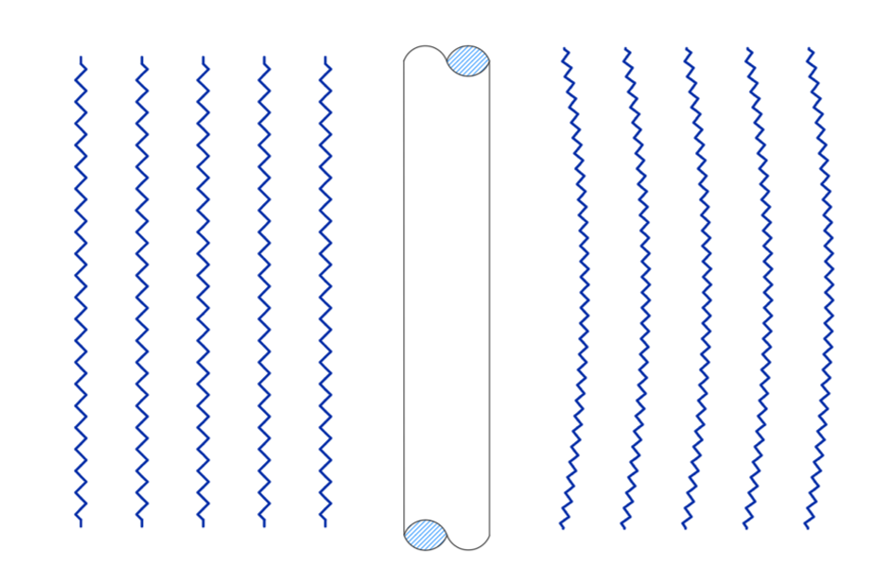
\includegraphics[width=16cm]{Imagenes/ondaincidente3.png}
\caption{Onda incidente perturbada.}\label{fig:Onda perturbada}
\end{figure}
Si ahora aplicamos las ecuaciones de Maxwell a la situación ilustrada en la figura \ref{fig:Onda perturbada}, obtenemos:
\begin{equation}
\label{eq:Onda perturbada}
\begin{split}
\left.
\begin{aligned}
&\nabla\cdot D_1 = \rho_1\qquad & \nabla\times D_1 = -\varepsilon_1\frac{\partial B_1}{\partial t}\\
&\nabla\cdot B_1 = 0\qquad & \nabla\times B_1 = \mu_1 J_{f1}+\mu_1\frac{\partial D_1}{\partial t}
\end{aligned}
\right\}
\quad\text{En }\Omega_1\\
\left.
\begin{aligned}
&\nabla\cdot D_2 = \rho_2\qquad & \nabla\times D_2 = -\varepsilon_2\frac{\partial B_2}{\partial t}\\
&\nabla\cdot B_2 = 0\qquad & \nabla\times B_2 = \mu_2 J_{f2}+\mu_2\frac{\partial D_2}{\partial t}
\end{aligned}
\right\}
\quad\text{En }\Omega_2\\
\left. 
D_1\cdot n=D_2\cdot n \qquad \frac{B_1}{\mu_1}\cdot n=\frac{B_2}{\mu_2}\cdot n
\right\}
\quad\text{En }\Gamma\\
\end{split}
\end{equation}
Debemos tener en cuenta que las propiedades del microhilo tendrán un efecto sobre el campo incidente. En caso de que las propiedades del volumen $\Omega_1$ sean iguales a los de $\Omega_2$, esto es $\varepsilon_1=\varepsilon_2$ y $\mu_1=\mu_2$\footnote{Por conveniencia matemática dejaremos todo escrito en términos del campo $\Omega_2$}. La situación descrita se puede ilustrar como en la imagen \ref{fig:Onda no afectada} y se puede representar en las ecuaciones de Maxwell de la forma:
\begin{equation}
\label{eq:Onda no afectada}
\begin{split}
\left.
\begin{aligned}
&\nabla\cdot D_i = \rho_1\qquad & \nabla\times D_1 = -\varepsilon_2\frac{\partial B_i}{\partial t}\\
&\nabla\cdot B_i = 0\qquad & \nabla\times B_i = \mu_2 J_{f1}+\mu_2\frac{\partial D_i}{\partial t}
\end{aligned}
\right\}
\quad\text{En }\Omega_1\\
\left.
\begin{aligned}
&\nabla\cdot D_i = \rho_2\qquad & \nabla\times D_i = -\varepsilon_2\frac{\partial B_i}{\partial t}\\
&\nabla\cdot B_i = 0\qquad & \nabla\times B_i = \mu_2 J_{f2}+\mu_2\frac{\partial D_i}{\partial t}
\end{aligned}
\right\}
\quad\text{En }\Omega_2\\
\left. 
D_i\cdot n=D_i\cdot n \qquad \frac{B_i}{\mu_2}\cdot n=\frac{B_i}{\mu_2}\cdot n
\right\}
\quad\text{En }\Gamma\\
\end{split}
\end{equation}
\begin{figure}[H]
\centering
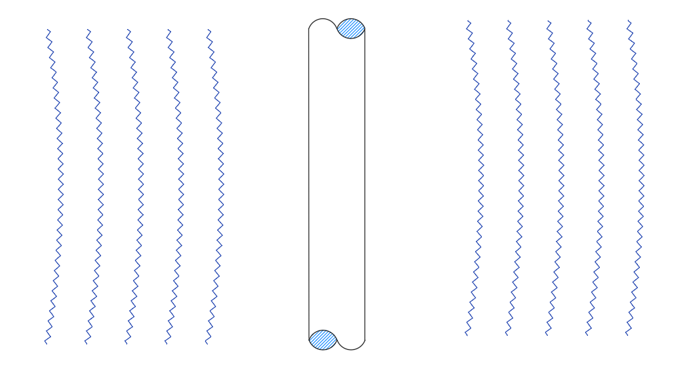
\includegraphics[width=16cm]{Imagenes/ondaincidente2.png}
\caption{Micro-hilo no tiene efecto sobre la onda.}\label{fig:Onda no afectada}
\end{figure}
Sabemos que en la situación expuesta en la ecuación \eqref{eq:Onda perturbada} el campo resultante, que es el expuesto en las ecuaciones puede verse como el campo incidente sumado al campo difundido producto del encuentro de la onda con al micro-hilo, por lo tanto los campos pueden ser representados como:
\begin{equation}
\label{eq:Descomposicion campos}
\begin{split}
D=D_i+D_d\\
B=B_i+B_d
\end{split}
\end{equation}
Donde $D_i$ y $B_i$ es el desplazamiento eléctrico inducido y $B_i$ es el campo magnético inducido.\\
Es correcto asumir que en nuestro sistema no hay corrientes electricas ni densidad de corriente por lo tanto los terminos de $\rho$ y $\vec{J}$ pueden ser eliminados. Por lo tanto podemos reescribir la ecuación \eqref{eq:Onda perturbada} como:
\begin{equation}
\label{eq:Onda perturbada y separada}
\begin{split}
\left.
\begin{aligned}
&\nabla\cdot D_{1d} + \nabla\cdot D_{i} = 0\qquad & \nabla\times D_{1d}+\nabla\times D_i = -\varepsilon_1\left(\frac{\partial B_{1d}}{\partial t}+\frac{\partial B_i}{\partial t}\right)\\
&\nabla\cdot B_{1d} +\nabla\cdot B_i = 0\qquad &  \nabla\times B_{1d}+\nabla\times B_i = \mu_1\left(\frac{\partial D_{1d}}{\partial t}+\frac{\partial D_i}{\partial t}\right)
\end{aligned}
\right\}
\quad\text{En }\Omega_1\\
\left.
\begin{aligned}
&\nabla\cdot D_{2d} + \nabla\cdot D_{i} = 0\qquad & \nabla\times D_{2d}+\nabla\times D_i = -\varepsilon_2\left(\frac{\partial B_{2d}}{\partial t}+\frac{\partial B_i}{\partial t}\right)\\
&\nabla\cdot B_{2d} +\nabla\cdot B_i = 0\qquad &  \nabla\times B_{2d}+\nabla\times B_i = \mu_2\left(\frac{\partial D_{2d}}{\partial t}+\frac{\partial D_i}{\partial t}\right)
\end{aligned}
\right\}
\quad\text{En }\Omega_2\\
\left. 
D_1\cdot n=D_2\cdot n \qquad \frac{B_1}{\mu_1}\cdot n=\frac{B_2}{\mu_2}\cdot n
\right\}
\quad\text{En }\Gamma\\
\end{split}
\end{equation}
Entonces si solo quisieramos saber como se comporta la onda difundida, solo es necesario restar la ecuación \eqref{eq:Onda no afectada} a la ecuación \eqref{eq:Onda perturbada y separada}:
\begin{equation}
\label{eq:Ondas restadas}
\begin{split}
\left.
\begin{aligned}
&\nabla\cdot D_{1d}= 0\qquad & \nabla\times D_{1d}= -\varepsilon_1\frac{\partial B_{1d}}{\partial t}-(\varepsilon_1-\varepsilon	_2)\frac{\partial B_i}{\partial t}\\
&\nabla\cdot B_{1d} = 0\qquad &  \nabla\times B_{1d}= \mu_1\frac{\partial D_{1d}}{\partial t}+(\mu_1-\mu_2)\frac{\partial D_i}{\partial t}
\end{aligned}
\right\}
\quad\text{En }\Omega_1\\
\left.
\begin{aligned}
&\nabla\cdot D_{1d}= 0\qquad & \nabla\times D_{1d}= -\varepsilon_1\frac{\partial B_{1d}}{\partial t}\\
&\nabla\cdot B_{1d} = 0\qquad &  \nabla\times B_{1d}= \mu_1\frac{\partial D_{1d}}{\partial t}
\end{aligned}
\right\}
\quad\text{En }\Omega_2\\
\left. 
D_{1d}\cdot n=D_{2d}\cdot n \qquad \left(\frac{1}{\mu_1}B_{1d}\cdot n-\frac{1}{\mu_2}B_{2d}\cdot n\right)=\left(\frac{1}{\mu_2}-\frac{1}{\mu_1}\right)B_i\cdot n
\right\}
\quad\text{En }\Gamma\\
\end{split}
\end{equation}
Se puede asumir una onda armónica con frecuencia $\omega$ para representar el desplazamiento eléctrico y el campo magnético:
$$B(x,t)=B(x)e^{i\omega t}$$
$$D(x,t)=D(x)e^{i\omega t}$$
La ecuación \eqref{eq:Ondas restadas} queda:
\begin{equation}
\label{eq:Ondas armonicas restadas }
\begin{split}
\left.
\begin{aligned}
&\nabla\cdot D_{1d}= 0\qquad & \nabla\times D_{1d}= -\varepsilon_1i\omega_d B_{1d}-(\varepsilon_1-\varepsilon	_2) i\omega_i B_i\\
&\nabla\cdot B_{1d} = 0\qquad &  \nabla\times B_{1d}= \mu_1 i\omega_d D_{1d}+(\mu_1-\mu_2)i\omega_i D_i
\end{aligned}
\right\}
\quad\text{En }\Omega_1\\
\left.
\begin{aligned}
&\nabla\cdot D_{1d}= 0\qquad & \nabla\times D_{1d}= -\varepsilon_1 i\omega_d B_{1d}\\
&\nabla\cdot B_{1d} = 0\qquad &  \nabla\times B_{1d}= \mu_1 i\omega_d D_{1d}
\end{aligned}
\right\}
\quad\text{En }\Omega_2\\
\left. 
D_{1d}\cdot n=D_{2d}\cdot n \qquad \left(\frac{1}{\mu_1}B_{1d}\cdot n-\frac{1}{\mu_2}B_{2d}\cdot n\right)=\left(\frac{1}{\mu_2}-\frac{1}{\mu_1}\right)B_i\cdot n
\right\}
\quad\text{En }\Gamma\\
\end{split}
\end{equation}
Al ser la onda incidente de una longitud de onda muy grande con respecto al cilindro es correcto asumir que $\lambda_i\rightarrow\infty$. Sabemos que por definición $w=v/\lambda$, por lo tanto $w_i\rightarrow 0$. Podemos escribir las cantidades auxiliares:
\begin{equation}
\begin{gathered}
\begin{aligned}
b_s=\sqrt{\varepsilon_2}B_s\\
d_s=\sqrt{\mu_2}D_s\\
x'=\frac{x}{d_x}
\end{aligned}
\end{gathered}
\end{equation}
A partir de esto podemos reescribir la ecuación \eqref{eq:Ondas armonicas restadas } utiliando las nuevas cantidades auxiliares:
\begin{equation}
\label{eq:Ondas armonicas restadas con cantidades auxiliares}
\begin{split}
\left.
\begin{aligned}
&\nabla\cdot d_{1d}= 0\qquad & \nabla\times d_{1d}= \frac{\varepsilon_1}{\varepsilon_2}i\beta b_{1d}\\
&\nabla\cdot b_{1d} = 0\qquad &  \nabla\times b_{1d}=\frac{\mu_1}{\mu_2}i\beta d_{1d}
\end{aligned}
\right\}
\quad\text{En }\Omega_1\\
\left.
\begin{aligned}
&\nabla\cdot d_{1d}= 0\qquad & \nabla\times d_{1d}= -i\beta b_{1d}\\
&\nabla\cdot b_{1d} = 0\qquad &  \nabla\times b_{1d}= i\beta d_{1d}
\end{aligned}
\right\}
\quad\text{En }\Omega_2\\
\left. 
d_{1d}\cdot n=d_{2d}\cdot n \qquad \left(\frac{1}{\mu_1}b_{1d}\cdot n-\frac{1}{\mu_2}b_{2d}\cdot n\right)=\left(\frac{1}{\mu_2}-\frac{1}{\mu_1}\right)b_i\cdot n
\right\}
\quad\text{En }\Gamma\\
\end{split}
\end{equation}
Con $\beta=wd\sqrt{\varepsilon_2\mu_2}$. Podemos expandir $d$ y $b$, utilizando $\beta$ como:
\begin{equation}
\begin{gathered}
d=d_s^{(0)}+\beta d_s^{(1)}+\beta^2 d_s^{(2)}...\\
b=b_s^{(0)}+\beta b_s^{(1)}+\beta^2 b_s^{(2)}...\\
\end{gathered}
\end{equation}
Y ahora considerando los términos de orden cero de la ecuación \eqref{eq:Ondas armonicas restadas con cantidades auxiliares}, escribimos solo los términos del campo mágnetico:
\begin{equation}
\label{eq:Sistema Campo Magnetico}
\begin{gathered}
\begin{aligned}
&\nabla\cdot b_{1d}^{(0)}= 0\qquad & \nabla\times b_{1d}^{(0)}= 0\\
&\nabla\cdot b_{2d}^{(0)} = 0\qquad &  \nabla\times b_{2d}^{(0)}= 0\\
\end{aligned}\\
\left(\frac{1}{\mu_1}b_{1d}^{(0)}\cdot n-\frac{1}{\mu_2}b_{2d}^{(0)}\cdot n\right)=\left(\frac{1}{\mu_2}-\frac{1}{\mu_1}\right)b_i\cdot n
%\quad\text{En }\Gamma
\end{gathered}
\end{equation}
Aplicando el operador $\nabla$ a las ecuaciones en $\Omega$ podemos concluir que:
\begin{itemize}
\item Por la identidad de la divergencia de un rotor:
\begin{equation*}
\begin{split}
\nabla \cdot (\nabla \times B_{1d}^{(0)})=0\\
\nabla \cdot (\nabla \times B_{2d}^{(0)})=0\\
\end{split}
\end{equation*}
Podemos determinar 	que los campos $B_{1d}$ y $B_{2d}$ son convervativos basandonos en que el rotor en ambos casos es cero, esto quiere decir que hay una función potencial que puede describir el comportamiento del campo.
\item Denominaremos como $\psi$ a la función escalar potencial que describirá nuestros campos:
$$\nabla \cdot \varphi = B_{d}$$
\item Nuevamente aplicamos el operador $\nabla$ pero esta vez en los gradientes del campo y utilizando la nueva notación con $\varphi$, notar que estas ecuaciones se cumplen para el campo en $\Omega_1$ y $\Omega_2$ respectivamente:
$$\nabla^2\cdot \varphi_{1d}=0$$
$$\nabla^2\cdot \varphi_{2d}=0$$
\item Reescribimos las ecuaciones en el borde $\Gamma$ y añadimos una más:
$$\left(\frac{1}{\mu_1}\frac{\partial \varphi_{1d}}{\partial n}-\frac{1}{\mu_2}\frac{\partial \varphi_{2d}}{\partial n}\right)=\left(\frac{1}{\mu_2}-\frac{1}{\mu_1}\right)\frac{\partial \varphi_{i}}{\partial n}$$
$$\varphi_{1d}=\varphi_{2d}\qquad\text{En la frontera }\Gamma$$
\end{itemize}
Finalmente nos encontramos con una ecuación diferencial con condiciones de borde, justamente lo necesario para resolver este problema utilizando el método de elementos de borde.

\begin{equation}
\label{eq:Ecuacion del problema}
\boxed{
\begin{gathered}
\nabla^2\cdot \varphi_{1d}=0,\qquad\nabla^2\cdot \varphi_{2d}=0\qquad\text{En }\Omega_1,\Omega_2\\
\left(\frac{1}{\mu_1}\frac{\partial \varphi_{1d}}{\partial n}-\frac{1}{\mu_2}\frac{\partial \varphi_{2d}}{\partial n}\right)=\left(\frac{1}{\mu_2}-\frac{1}{\mu_1}\right)\frac{\partial \varphi_{i}}{\partial n}\qquad\varphi_{1d}=\varphi_{2d}\qquad\text{En la frontera }\Gamma\\
\end{gathered}
}
\end{equation}
Y como se vio en la sección \ref{sec:BEM.} la ecuación \eqref{eq:Ecuacion del problema} puede representarse por una formulación de elementos de borde como:
\begin{equation}
\label{eq:Ecuacion con operadores sin condiciones}
\begin{gathered}
\frac{1}{2}\varphi_{1d}+K\cdot\varphi_{1d}-V\left(\frac{\partial}{\partial n}\varphi_{1d}\right)=0\\
\frac{1}{2}\varphi_{1d}-K\cdot\varphi_{1d}+V\left(\frac{\partial}{\partial n}\varphi_{2d}\right)=0\\
\text{En la frontera }\Gamma
\end{gathered}
\end{equation}
La primera ecuación presente en el conjunto mostrado en \eqref{eq:Ecuacion con operadores sin condiciones} es del mismo desarrollo que el mostrado en la sección citada. Sin embargo la segunda ecuación tiene los signos invertidos debido a que las normales apuntan en sentido contrario, $ergo$ los signos de los términos en donde las normales tienen incidencia deben tener distinto signo para que ambas tengan la misma convención de signos. Si además a lo anterior se aplican las condiciones de borde de \eqref{eq:Ecuacion del problema}:
\begin{equation}
\label{eq:Ecuacion de borde con condiciones de borde}
\begin{gathered}
\frac{1}{2}\varphi_{1d}+K\cdot\varphi_{1d}-V\left(\frac{\partial}{\partial n}\varphi_{1d}\right)=0\\
\frac{1}{2}\varphi_{2d}-K\cdot\varphi_{1d}+\mu_2 V\left(\frac{1}{\mu_1}\frac{\partial}{\partial n}\varphi_{1d}-\left(\frac{1}{\mu_2}-\frac{1}{\mu_1}\right)\frac{\partial}{\partial n}\varphi_{i}\right)=0\\
\text{En la frontera }\Gamma
\end{gathered}
\end{equation}
La forma matricial de la ecuación \eqref{eq:Ecuacion de borde con condiciones de borde} es:
\begin{equation}\label{eq:Forma matricial ecuacion 1}
\begin{bmatrix}
\frac{1}{2}I+K & -V \\ 
\frac{1}{2}I-K & \frac{\mu_2}{\mu_1}V
\end{bmatrix}
\begin{bmatrix}
\varphi_{1d}\\ 
\frac{\partial}{\partial n}\varphi_{1d}
\end{bmatrix}
=\begin{bmatrix}
0\\ 
\frac{\mu_1-\mu_2}{\mu_1}\frac{\partial \varphi_i}{\partial n}
\end{bmatrix}
\end{equation}
Donde $I$ sería la matriz identidad. Usando los mismos pasos matemáticos pero teniendo como 'campos iniciales' el campo eléctrico $E$ y la intensidad de campo magnético $H$ podemos llegar a una ecuación que tiene la misma estructura pero distintos coeficientes:
\begin{equation}
\begin{bmatrix}
\frac{1}{2}I+K & -V \\ 
\frac{1}{2}I-K & \frac{\varepsilon_1}{\varepsilon_2}V
\end{bmatrix}
\begin{bmatrix}
\varphi_{1d}\\ 
\frac{\partial}{\partial n}\varphi_{1d}
\end{bmatrix}
=\begin{bmatrix}
0\\ 
\frac{\varepsilon_2-\varepsilon_1}{\varepsilon_2}\frac{\partial \varphi_i}{\partial n}
\end{bmatrix}
\end{equation}
\section{Creación de mallas.}\label{sec:Creacion de mallas.}
Como se ha dicho en la sección \ref{sec:Biblioteca bempp.} es necesario una malla de estudio, a la cual aplicaremos las condiciones del problema. Corresponde utilizar el formato aceptado por la librería, $".msh"$. La creación de la geomtería de la malla se hace en el Software $SolidWorks$ cite{Fulkerson SolidWorks} en  donde se exporta el archivo en formato $STEP$:
\begin{figure}[H]
\centering
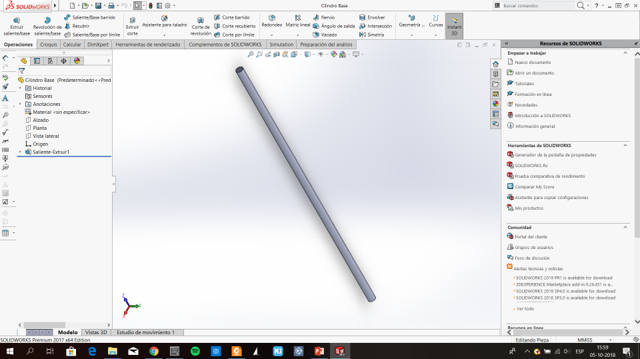
\includegraphics[scale=0.8]{Imagenes/Cilindro STEP.png}
\caption{Cilindro en SolidWorks}
\end{figure}
Luego, este archivo en formato $STEP$ se abre en el software $Gmsh$, el cual nos permitirá editar la forma de la malla, tamaño de los elementos, forma de los elementos, etc. Las mallas utilizadas tienen la forma de las imagenes que se muestran en \ref{fig:malla1}, \ref{fig:malla2} y \ref{fig:malla3}, cambiando el tamaño del elemento:
\begin{figure}[H]
\centering
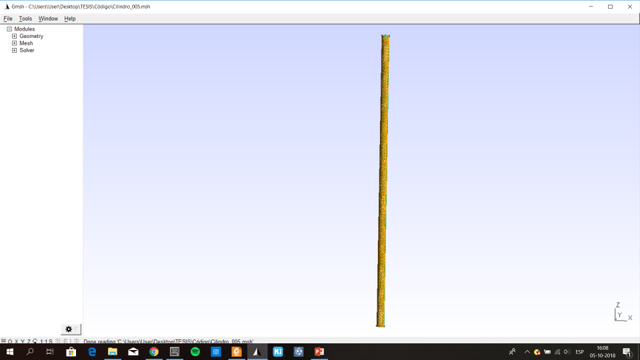
\includegraphics[scale=0.8]{Imagenes/malla1.png}
\caption{Malla vista completa}\label{fig:malla1}
\end{figure}
\begin{figure}[H]
\centering
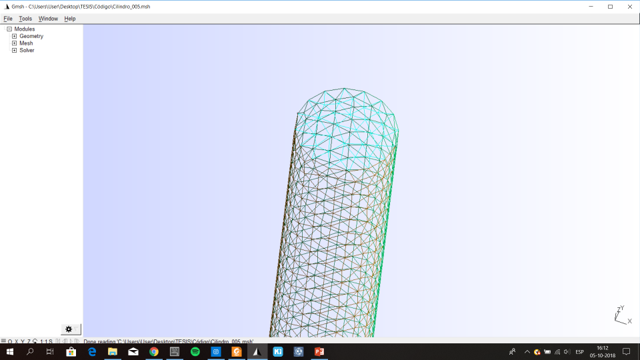
\includegraphics[scale=0.8]{Imagenes/malla2.png}
\caption{Malla detalle tapa}\label{fig:malla2}
\end{figure}
\begin{figure}[H]
\centering
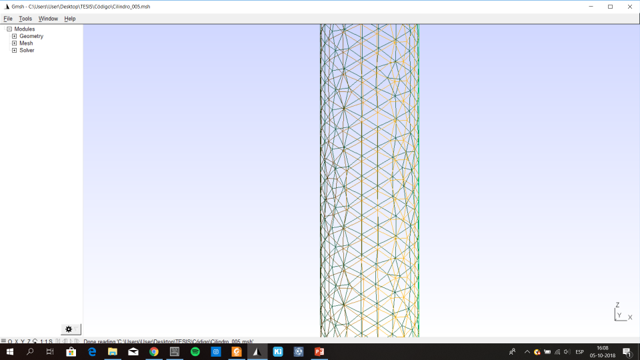
\includegraphics[scale=0.8]{Imagenes/malla3.png}
\caption{Malla detalle elementos}\label{fig:malla3}
\end{figure}
En el software $Gmsh$ también es posible verificar la dirección de los vectores normales y tangentes, por medio de inspección visual. Esto no es suficiente, por lo que abrimos la malla en $MeshLab$\cite{Meshlab} y verificamos no solo los puntos anteriores, sino también:
\begin{itemize}
\item Geometrías bien ubicadas.
\item Vectores normales en la dirección deseada.
\item Caras no duplicadas.
\end{itemize}
INSERTAR IMAGEN DE LA MALLA EN MESHLAB
\section{Desarrollo del problema.}
\setcounter{figure}{0}
\setcounter{equation}{0}
Como bien hablamos en capítulos anteriores, la resolución de la problematica planteada se realizará bajo la plataforma de $Jupyter\text{ }Notebook$. \\
Es importante partir comenzar importando librerías que serán necesarias para la resolución de los problemas, obviamente tenemos a $bempp$ y a $numpy$, una librería fundamental de python que contiene funciones de algebra lineal y arreglos de N-dimensiones que son utilizadas en todo método de resolución de ecuaciones diferenciales. Además de esto, se definen los nodos utilizados para realizar la cuadratura de Gauss.
\begin{tcolorbox}
\begin{Verbatim}[commandchars=\\\{\}]
\PY{c+c1}{\PYZsh{} Import libraries}
\PY{k+kn}{import} \PY{n+nn}{bempp}\PY{n+nn}{.}\PY{n+nn}{api}
\PY{k+kn}{import} \PY{n+nn}{numpy} \PY{k}{as} \PY{n+nn}{np}
\PY{n}{bempp}\PY{o}{.}\PY{n}{api}\PY{o}{.}\PY{n}{set\PYZus{}ipython\PYZus{}notebook\PYZus{}viewer}\PY{p}{(}\PY{p}{)}

\PY{c+c1}{\PYZsh{} Set quadrature options}        
\PY{n}{bempp}\PY{o}{.}\PY{n}{api}\PY{o}{.}\PY{n}{global\PYZus{}parameters}\PY{o}{.}\PY{n}{quadrature}\PY{o}{.}\PY{n}{near}\PY{o}{.}\PY{n}{double\PYZus{}order} \PY{o}{=} \PY{l+m+mi}{4}
\PY{n}{bempp}\PY{o}{.}\PY{n}{api}\PY{o}{.}\PY{n}{global\PYZus{}parameters}\PY{o}{.}\PY{n}{quadrature}\PY{o}{.}\PY{n}{medium}\PY{o}{.}\PY{n}{double\PYZus{}order} \PY{o}{=} \PY{l+m+mi}{4}
\PY{n}{bempp}\PY{o}{.}\PY{n}{api}\PY{o}{.}\PY{n}{global\PYZus{}parameters}\PY{o}{.}\PY{n}{quadrature}\PY{o}{.}\PY{n}{far}\PY{o}{.}\PY{n}{double\PYZus{}order} \PY{o}{=} \PY{l+m+mi}{4}
\end{Verbatim}
\end{tcolorbox}
Se define la malla, la cual es importada y creada como se explica en la subsección \ref{sec:Creacion de mallas.}. Se imprime la cantidad de elementos de la malla, lo que nos permitirá saber el tamaño de la matriz que resolveremos. Graficaremos la malla utilizando el comando $plot$, el cual grafica bajo la librería $plotly$, librería de gráficas de python y que nos permite revisar la gráfica de nuestra malla a mayor profundida. Sin embargo, por sus ajustes por defecto la malla puede verse algo rara, pero es solo un efecto óptico. 

\begin{tcolorbox}
\begin{Verbatim}[commandchars=\\\{\}]
\PY{c+c1}{\PYZsh{} Define grid}
\PY{n}{grid} \PY{o}{=} \PY{n}{bempp}\PY{o}{.}\PY{n}{api}\PY{o}{.}\PY{n}{import\PYZus{}grid}\PY{p}{(}\PY{l+s+s2}{\PYZdq{}}\PY{l+s+s2}{Cilindro\PYZus{}005.msh}\PY{l+s+s2}{\PYZdq{}}\PY{p}{)}

\PY{c+c1}{\PYZsh{} Print out the number of elements}
\PY{n}{number\PYZus{}of\PYZus{}elements} \PY{o}{=} \PY{n}{grid}\PY{o}{.}\PY{n}{leaf\PYZus{}view}\PY{o}{.}\PY{n}{entity\PYZus{}count}\PY{p}{(}\PY{l+m+mi}{0}\PY{p}{)}    
\PY{n+nb}{print}\PY{p}{(}\PY{l+s+s2}{\PYZdq{}}\PY{l+s+s2}{The grid has }\PY{l+s+si}{\PYZob{}0\PYZcb{}}\PY{l+s+s2}{ elements.}\PY{l+s+s2}{\PYZdq{}}\PY{o}{.}\PY{n}{format}\PY{p}{(}\PY{n}{number\PYZus{}of\PYZus{}elements}\PY{p}{)}\PY{p}{)}

\PY{c+c1}{\PYZsh{} Plot the grid}
\PY{n}{grid.plot()}
\end{Verbatim}
\end{tcolorbox}
\begin{figure}[H]
\centering
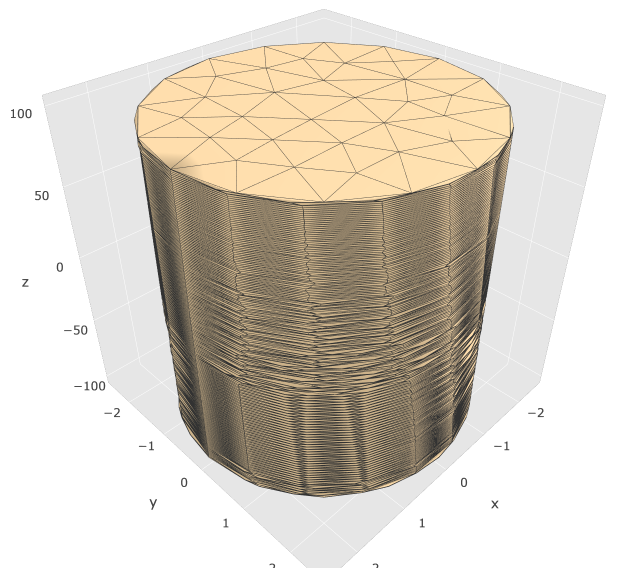
\includegraphics[scale=0.9]{Imagenes/graficas/Situacion 1/Malla/malla 1.png} 
\caption{Malla con ajustes predeterminados en $plotly$}
\end{figure}
\begin{figure}[H]
\centering
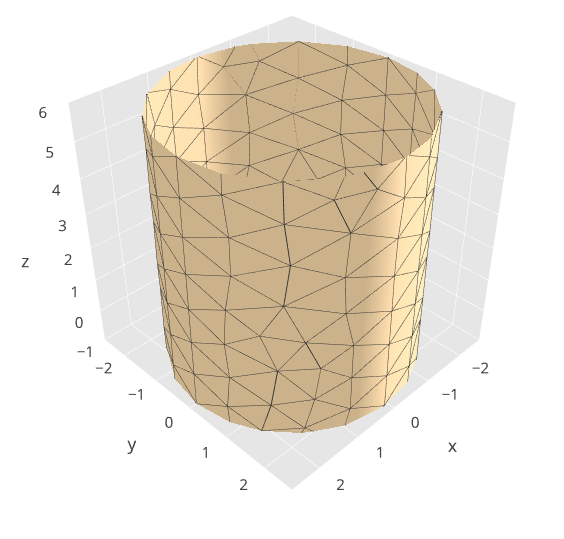
\includegraphics[scale=0.8]{Imagenes/graficas/Situacion 1/Malla/malla 2.png} 
\caption{Malla con eje $z$ no 'comprimido' en $plotly$}
\end{figure}
El siguiente paso a seguir es crear los espacios de funciones, en este caso se ha dejado como una variable el orden de los espacios. Se imprime el valor del grado de libertad del espacio. \\
Se ingresan los datos del problemas.
\begin{tcolorbox}
\begin{Verbatim}[commandchars=\\\{\}]
\PY{c+c1}{\PYZsh{} Set the Dirichlet and Neumann orders}
\PY{n}{order\PYZus{}neumann} \PY{o}{=} \PY{l+m+mi}{0}
\PY{n}{order\PYZus{}dirichlet} \PY{o}{=} \PY{l+m+mi}{0}
 
 \PY{c+c1}{\PYZsh{} Create function spaces}       
\PY{n}{global\PYZus{}neumann\PYZus{}space} \PY{o}{=} \PY{n}{bempp}\PY{o}{.}\PY{n}{api}\PY{o}{.}\PY{n}{function\PYZus{}space}\PY{p}{(}\PY{n}{grid}\PY{p}{,} \PY{l+s+s2}{\PYZdq{}}\PY{l+s+s2}{DP}\PY{l+s+s2}{\PYZdq{}}\PY{p}{,} \PY{n}{order\PYZus{}neumann}\PY{p}{)}
\PY{n}{global\PYZus{}dirichlet\PYZus{}space} \PY{o}{=} \PY{n}{bempp}\PY{o}{.}\PY{n}{api}\PY{o}{.}\PY{n}{function\PYZus{}space}\PY{p}{(}\PY{n}{grid}\PY{p}{,} \PY{l+s+s2}{\PYZdq{}}\PY{l+s+s2}{DP}\PY{l+s+s2}{\PYZdq{}}\PY{p}{,} \PY{n}{order\PYZus{}dirichlet}\PY{p}{)}   
\PY{n}{NS} \PY{o}{=} \PY{n}{global\PYZus{}neumann\PYZus{}space}
\PY{n}{DS} \PY{o}{=} \PY{n}{global\PYZus{}dirichlet\PYZus{}space}

\PY{c+c1}{\PYZsh{} Print out the degrees of freedom}        
\PY{n+nb}{print}\PY{p}{(}\PY{l+s+s2}{\PYZdq{}}\PY{l+s+s2}{BEM dofs: }\PY{l+s+si}{\PYZob{}0\PYZcb{}}\PY{l+s+s2}{\PYZdq{}}\PY{o}{.}\PY{n}{format}\PY{p}{(}\PY{n}{NS}\PY{o}{.}\PY{n}{global\PYZus{}dof\PYZus{}count}\PY{p}{)}\PY{p}{)}

\PY{c+c1}{\PYZsh{}Preambulo}

\PY{n}{omega} \PY{o}{=} \PY{l+m+mf}{2.}\PY{o}{*}\PY{n}{np}\PY{o}{.}\PY{n}{pi}\PY{o}{*}\PY{l+m+mf}{10.e9}
\PY{n}{e0} \PY{o}{=} \PY{l+m+mf}{8.854}\PY{o}{*}\PY{l+m+mf}{1e\PYZhy{}12}\PY{o}{*}\PY{l+m+mf}{1e\PYZhy{}18}
\PY{n}{mu0} \PY{o}{=} \PY{l+m+mf}{4.}\PY{o}{*}\PY{n}{np}\PY{o}{.}\PY{n}{pi}\PY{o}{*}\PY{l+m+mf}{1e\PYZhy{}7}\PY{o}{*}\PY{l+m+mf}{1e6}
\PY{n}{mue} \PY{o}{=} \PY{p}{(}\PY{l+m+mf}{1.}\PY{p}{)}\PY{o}{*}\PY{n}{mu0}
\PY{n}{ee} \PY{o}{=} \PY{p}{(}\PY{l+m+mf}{16.}\PY{p}{)}\PY{o}{*}\PY{n}{e0}
\PY{n}{mui} \PY{o}{=} \PY{p}{(}\PY{o}{\PYZhy{}}\PY{l+m+mf}{2.9214}\PY{o}{+}\PY{l+m+mf}{0.5895}\PY{n}{j}\PY{p}{)}\PY{o}{*}\PY{n}{mu0}
\PY{n}{ei} \PY{o}{=} \PY{p}{(}\PY{l+m+mf}{82629.2677}\PY{o}{\PYZhy{}}\PY{l+m+mf}{200138.2211}\PY{n}{j}\PY{p}{)}\PY{o}{*}\PY{n}{e0}
\PY{n}{k} \PY{o}{=} \PY{n}{omega}\PY{o}{*}\PY{n}{np}\PY{o}{.}\PY{n}{sqrt}\PY{p}{(}\PY{n}{e0}\PY{o}{*}\PY{n}{mu0}\PY{p}{)}
\PY{n}{lam} \PY{o}{=} \PY{l+m+mi}{2}\PY{o}{*}\PY{n}{np}\PY{o}{.}\PY{n}{pi}\PY{o}{/}\PY{n}{k}
\end{Verbatim}
\end{tcolorbox}
Se generan los operadores que están presentes en la ecuación \eqref{eq:Forma matricial ecuacion 1}. Es importantehacer notar que el comando $blocked$ genera una matriz capaz de almacenar operadores, este será el lado izquierdo de la ecuación.
\begin{tcolorbox}
\begin{Verbatim}[commandchars=\\\{\}]
\PY{c+c1}{\PYZsh{}Operators}
\PY{n}{slp} \PY{o}{=} \PY{n}{bempp}\PY{o}{.}\PY{n}{api}\PY{o}{.}\PY{n}{operators}\PY{o}{.}\PY{n}{boundary}\PY{o}{.}\PY{n}{laplace}\PY{o}{.}\PY{n}{single\PYZus{}layer}\PY{p}{(}\PY{n}{NS}\PY{p}{,}\PY{n}{DS}\PY{p}{,}\PY{n}{DS}\PY{p}{)}
\PY{n}{dlp} \PY{o}{=} \PY{n}{bempp}\PY{o}{.}\PY{n}{api}\PY{o}{.}\PY{n}{operators}\PY{o}{.}\PY{n}{boundary}\PY{o}{.}\PY{n}{laplace}\PY{o}{.}\PY{n}{double\PYZus{}layer}\PY{p}{(}\PY{n}{DS}\PY{p}{,}\PY{n}{DS}\PY{p}{,}\PY{n}{DS}\PY{p}{)}        
\PY{n}{id} \PY{o}{=} \PY{n}{bempp}\PY{o}{.}\PY{n}{api}\PY{o}{.}\PY{n}{operators}\PY{o}{.}\PY{n}{boundary}\PY{o}{.}\PY{n}{sparse}\PY{o}{.}\PY{n}{identity}\PY{p}{(}\PY{n}{DS}\PY{p}{,}\PY{n}{DS}\PY{p}{,}\PY{n}{DS}\PY{p}{)}
                
\PY{c+c1}{\PYZsh{}Formation of the left hand side matrix}
\PY{n}{blocked} \PY{o}{=} \PY{n}{bempp}\PY{o}{.}\PY{n}{api}\PY{o}{.}\PY{n}{BlockedOperator}\PY{p}{(}\PY{l+m+mi}{2}\PY{p}{,} \PY{l+m+mi}{2}\PY{p}{)}
\PY{n}{blocked}\PY{p}{[}\PY{l+m+mi}{0}\PY{p}{,} \PY{l+m+mi}{0}\PY{p}{]} \PY{o}{=} \PY{l+m+mf}{0.5} \PY{o}{*} \PY{n+nb}{id} \PY{o}{+} \PY{n}{dlp}
\PY{n}{blocked}\PY{p}{[}\PY{l+m+mi}{0}\PY{p}{,} \PY{l+m+mi}{1}\PY{p}{]} \PY{o}{=} \PY{o}{\PYZhy{}}\PY{n}{slp}
\PY{n}{blocked}\PY{p}{[}\PY{l+m+mi}{1}\PY{p}{,} \PY{l+m+mi}{0}\PY{p}{]} \PY{o}{=} \PY{l+m+mf}{0.5} \PY{o}{*} \PY{n+nb}{id} \PY{o}{\PYZhy{}} \PY{n}{dlp}
\PY{n}{blocked}\PY{p}{[}\PY{l+m+mi}{1}\PY{p}{,} \PY{l+m+mi}{1}\PY{p}{]} \PY{o}{=} \PY{n}{ep1}\PY{o}{/}\PY{n}{ep2} \PY{o}{*} \PY{n}{slp}
\end{Verbatim}
\end{tcolorbox}
El lado derecho de la ecuación está definido como una concatenación de dos funciones, que en el caso de la ecuación \eqref{eq:Forma matricial ecuacion 1} estás funciones son $0$ y $\frac{\partial \varphi_i}{\partial n}$, al definir $\varphi=e^{jkx}$ se puede representar su derivada en la normal como se presenta a continuación. Además estás funciones, recordemos, viven en un espacio de funciones que hemos definido más arriba, por lo que se debe definir la función dentro del espacio correspondiente para generar la 'función de malla':
\begin{tcolorbox}
\begin{Verbatim}[commandchars=\\\{\}]
\PY{c+c1}{\PYZsh{}Definition of functions}
\PY{k}{def} \PY{n+nf}{funcion1}\PY{p}{(}\PY{n}{x}\PY{p}{,} \PY{n}{n}\PY{p}{,} \PY{n}{domain\PYZus{}index}\PY{p}{,} \PY{n}{result}\PY{p}{)}\PY{p}{:}
\PY{n}{result}\PY{p}{[}\PY{p}{:}\PY{p}{]} \PY{o}{=} \PY{p}{(}\PY{p}{(}\PY{n}{ep2} \PY{o}{\PYZhy{}} \PY{n}{ep1}\PY{p}{)} \PY{o}{/} \PY{n}{ep2}\PY{p}{)} \PY{o}{*} \PY{p}{(}\PY{l+m+mf}{1.} \PY{o}{*} \PY{l+m+mi}{1}\PY{n}{j} \PY{o}{*} \PY{n}{k} \PY{o}{*} \PY{n}{n}\PY{p}{[}\PY{l+m+mi}{0}\PY{p}{]} \PY{o}{*} \PY{n}{np}\PY{o}{.}\PY{n}{exp}\PY{p}{(}\PY{l+m+mi}{1}\PY{n}{j} \PY{o}{*} \PY{n}{k} \PY{o}{*} \PY{n}{x}\PY{p}{[}\PY{l+m+mi}{0}\PY{p}{]}\PY{p}{)}\PY{p}{)}
\PY{n}{result}\PY{p}{[}\PY{p}{:}\PY{p}{]} \PY{o}{=} \PY{p}{(} Amp * n[0]\PY{p}{)}
        
\PY{k}{def} \PY{n+nf}{cero}\PY{p}{(}\PY{n}{x}\PY{p}{,} \PY{n}{n}\PY{p}{,} \PY{n}{domain\PYZus{}index}\PY{p}{,} \PY{n}{result}\PY{p}{)}\PY{p}{:}
\PY{n}{result}\PY{p}{[}\PY{p}{:}\PY{p}{]} \PY{o}{=} \PY{l+m+mi}{0}

\PY{c+c1}{\PYZsh{}Formation functions in the space}            
\PY{n}{funcion\PYZus{}fun} \PY{o}{=} \PY{n}{bempp}\PY{o}{.}\PY{n}{api}\PY{o}{.}\PY{n}{GridFunction}\PY{p}{(}\PY{n}{DS}\PY{p}{,} \PY{n}{fun}\PY{o}{=}\PY{n}{funcion1}\PY{p}{)}        
\PY{n}{cero\PYZus{}fun} \PY{o}{=} \PY{n}{bempp}\PY{o}{.}\PY{n}{api}\PY{o}{.}\PY{n}{GridFunction}\PY{p}{(}\PY{n}{NS}\PY{p}{,} \PY{n}{fun}\PY{o}{=}\PY{n}{cero}\PY{p}{)}
\end{Verbatim}
\end{tcolorbox}
Para resolver el sistema de ecuaciones existen varias formas de hacerlo, con distinta rapidez, precisión, entre otros factores. En la mayoría podemos ver como converge la solución, la cantidad de iteraciones realizadas para llegar a esta y la precisión de la misma, que en este caso viene dedo por el ajuste $tol$. La discretización de ambos lados de la ecuación viene por el comando $use\_strong\_form$, lo cual puede relizarse separadamente, pero aumenta la cantidad de capacidad computacional necesaria.
\begin{tcolorbox}
\begin{Verbatim}[commandchars=\\\{\}]
\PY{c+c1}{\PYZsh{}Solving the matrix system}
\PY{n}{sol}\PY{p}{,} \PY{n}{info}\PY{p}{,} \PY{n}{it\PYZus{}count} \PY{o}{=} \PY{n}{bempp}\PY{o}{.}\PY{n}{api}\PY{o}{.}\PY{n}{linalg}\PY{o}{.}\PY{n}{gmres}\PY{p}{(}\PY{n}{blocked}\PY{p}{,} \PY{p}{[}\PY{n}{cero\PYZus{}fun}\PY{p}{,} \PY{n}{funcion\PYZus{}fun}\PY{p}{]}\PY{p}{,}
		\PY{n}{use\PYZus{}strong\PYZus{}form}\PY{o}{=}\PY{k+kc}{True}\PY{p}{,} \PY{n}{return\PYZus{}iteration\PYZus{}count}\PY{o}{=}\PY{k+kc}{True}\PY{p}{,} \PY{n}{tol}\PY{o}{=}\PY{l+m+mf}{1e\PYZhy{}3}\PY{p}{)}

\PY{c+c1}{\PYZsh{}Print number of iterations}         
\PY{n+nb}{print}\PY{p}{(}\PY{l+s+s2}{\PYZdq{}}\PY{l+s+s2}{The linear system was solved in }\PY{l+s+si}{\PYZob{}0\PYZcb{}}\PY{l+s+s2}{ iterations}\PY{l+s+s2}{\PYZdq{}}\PY{o}{.}\PY{n}{format}\PY{p}{(}\PY{n}{it\PYZus{}count}\PY{p}{)}\PY{p}{)}
\end{Verbatim}
\end{tcolorbox}
Cuando se resuelve el sistema de matrices, se obtiene '2' soluciones. Como vemos en la ecuación \eqref{eq:Forma matricial ecuacion 1} obtenemos $\varphi_1$ y $\frac{\partial \varphi_1}{\partial n}$, lo que visto en el código serían la $solution\_dirichl$ y $solution\_neumann$ respectivamente. Como nos interesa ver la forma de la onda disipada, graficamos esta onda, es decir, $solution\_dirichl$ en torno a nuestra malla de estudio.
\begin{tcolorbox}
\begin{Verbatim}[commandchars=\\\{\}]
\PY{c+c1}{\PYZsh{}Divide the solution} 
\PY{n}{solution\PYZus{}dirichl}\PY{p}{,} \PY{n}{solution\PYZus{}neumann} \PY{o}{=} \PY{n}{sol}

\PY{c+c1}{\PYZsh{}Plot the solution} 
\PY{n}{solution\PYZus{}dirichl}\PY{o}{.}\PY{n}{plot}\PY{p}{(}\PY{p}{)}
\end{Verbatim}
\end{tcolorbox}
\begin{figure}[H]
\centering
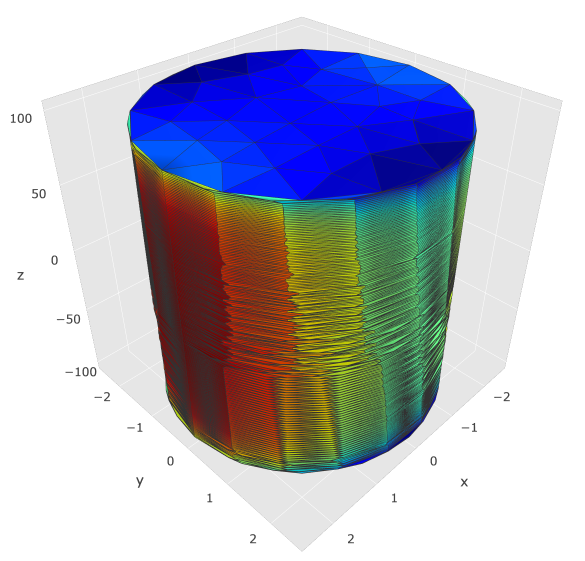
\includegraphics[width=16cm]{Imagenes/graficas/Situacion 1/Solucion ecuacion 1/3d.png}
\caption{Solución situacion 1}
\end{figure}

Además de ver la solución en 3D, se hace necesario ver en detalle que sucede el centro  de nuestra malla, por lo que generar una malla 2D sobre un plano $z$ determinado nos ayudaría a ver el comportamiento de la onda dentro de, en este caso, el cable.
\begin{tcolorbox}
\begin{Verbatim}[commandchars=\\\{\}]
\PY{c+c1}{\PYZsh{}Generate the grid} 
\PY{n}{n\PYZus{}grid\PYZus{}points} \PY{o}{=} \PY{l+m+mi}{200}
\PY{n}{xmin}\PY{p}{,} \PY{n}{xmax}\PY{p}{,} \PY{n}{ymin}\PY{p}{,} \PY{n}{ymax}\PY{o}{=}\PY{p}{[}\PY{o}{\PYZhy{}}\PY{l+m+mi}{3}\PY{p}{,}\PY{l+m+mi}{3}\PY{p}{,}\PY{o}{\PYZhy{}}\PY{l+m+mi}{3}\PY{p}{,}\PY{l+m+mi}{3}\PY{p}{]}
\PY{n}{plot\PYZus{}grid} \PY{o}{=} \PY{n}{np}\PY{o}{.}\PY{n}{mgrid}\PY{p}{[}\PY{n}{xmin}\PY{p}{:}\PY{n}{xmax}\PY{p}{:}\PY{n}{n\PYZus{}grid\PYZus{}points}\PY{o}{*}\PY{l+m+mi}{1}\PY{n}{j}\PY{p}{,}\PY{n}{ymin}\PY{p}{:}\PY{n}{ymax}\PY{p}{:}\PY{n}{n\PYZus{}grid\PYZus{}points}\PY{o}{*}\PY{l+m+mi}{1}\PY{n}{j}\PY{p}{]}
\PY{n}{points} \PY{o}{=} \PY{n}{np}\PY{o}{.}\PY{n}{vstack}\PY{p}{(}\PY{p}{(}\PY{n}{plot\PYZus{}grid}\PY{p}{[}\PY{l+m+mi}{0}\PY{p}{]}\PY{o}{.}\PY{n}{ravel}\PY{p}{(}\PY{p}{)}\PY{p}{,}
         \PY{n}{plot\PYZus{}grid}\PY{p}{[}\PY{l+m+mi}{1}\PY{p}{]}\PY{o}{.}\PY{n}{ravel}\PY{p}{(}\PY{p}{)}\PY{p}{,}
	 \PY{n}{np}\PY{o}{.}\PY{n}{zeros}\PY{p}{(}\PY{n}{plot\PYZus{}grid}\PY{p}{[}\PY{l+m+mi}{0}\PY{p}{]}\PY{o}{.}\PY{n}{size}\PY{p}{)}\PY{p}{)}\PY{p}{)}
\end{Verbatim}
\end{tcolorbox}

Se crean las funciones de espacio utilizando la malla en 3D.
\begin{tcolorbox}
\begin{Verbatim}[commandchars=\\\{\}]
\PY{c+c1}{\PYZsh{}Generate the spaces} 
\PY{n}{dp0\PYZus{}space} \PY{o}{=} \PY{n}{bempp}\PY{o}{.}\PY{n}{api}\PY{o}{.}\PY{n}{function\PYZus{}space}\PY{p}{(}\PY{n}{grid}\PY{p}{,} \PY{l+s+s2}{\PYZdq{}}\PY{l+s+s2}{DP}\PY{l+s+s2}{\PYZdq{}}\PY{p}{,} \PY{l+m+mi}{0}\PY{p}{)}
\PY{n}{p1\PYZus{}space} \PY{o}{=} \PY{n}{bempp}\PY{o}{.}\PY{n}{api}\PY{o}{.}\PY{n}{function\PYZus{}space}\PY{p}{(}\PY{n}{grid}\PY{p}{,} \PY{l+s+s2}{\PYZdq{}}\PY{l+s+s2}{DP}\PY{l+s+s2}{\PYZdq{}}\PY{p}{,} \PY{l+m+mi}{0}\PY{p}{)}
\end{Verbatim}
\end{tcolorbox}

Se generan los operadores bajo los puntos especificados en la malla 2D, es decir bajo un plano $z$ especificado.
\begin{tcolorbox}
\begin{Verbatim}[commandchars=\\\{\}]
\PY{c+c1}{\PYZsh{}Generate the operators} 
\PY{n}{slp\PYZus{}pot} \PY{o}{=} \PY{n}{bempp}\PY{o}{.}\PY{n}{api}\PY{o}{.}\PY{n}{operators}\PY{o}{.}\PY{n}{potential}\PY{o}{.}\PY{n}{laplace}\PY{o}{.}\PY{n}{single\PYZus{}layer}\PY{p}{(}\PY{n}{dp0\PYZus{}space}\PY{p}{,} \PY{n}{points}\PY{p}{)}
\PY{n}{dlp\PYZus{}pot} \PY{o}{=} \PY{n}{bempp}\PY{o}{.}\PY{n}{api}\PY{o}{.}\PY{n}{operators}\PY{o}{.}\PY{n}{potential}\PY{o}{.}\PY{n}{laplace}\PY{o}{.}\PY{n}{double\PYZus{}layer}\PY{p}{(}\PY{n}{p1\PYZus{}space}\PY{p}{,} \PY{n}{points}\PY{p}{)}
\end{Verbatim}
\end{tcolorbox}

Se evalua la solución en todos los puntos del plano, que vienen siendo los puntos internos de la malla en un plano especifico, es decir, se utiliza la ecuación \eqref{eq:Calculo puntos internos discretizada}.
\begin{tcolorbox}
\begin{Verbatim}[commandchars=\\\{\}]
\PY{c+c1}{\PYZsh{}Evaluation in internal points} 
\PY{n}{u\PYZus{}evaluated} \PY{o}{=} \PY{n}{slp\PYZus{}pot} \PY{o}{*} \PY{n}{solution\PYZus{}neumann} \PY{o}{\PYZhy{}} \PY{n}{dlp\PYZus{}pot} \PY{o}{*} \PY{n}{solution\PYZus{}dirichl}
\end{Verbatim}
\end{tcolorbox}
Finalmente se grafica la solución obtenida, en este caso obtendremos una solución con una parte imaginaria, a nosotros para graficar solo nos interesa la parte real de la solución por lo que filtraremos bajo este criterio. Otro criterio de filtro es que los resultados fuera de la malla, son irrelevantes, por lo que se eliminan. |
\begin{tcolorbox}
\begin{Verbatim}[commandchars=\\\{\}]
\PY{c+c1}{\PYZsh{} The next command ensures that plots are shown within the IPython notebook}
\PY{o}{\PYZpc{}}\PY{k}{matplotlib} inline                
\PY{k+kn}{from} \PY{n+nn}{matplotlib} \PY{k}{import} \PY{n}{pylab} \PY{k}{as} \PY{n}{plt}
         
\PY{c+c1}{\PYZsh{}Plot the results}       
\PY{n}{fig}\PY{p}{,}\PY{n}{ax} \PY{o}{=} \PY{n}{plt}\PY{o}{.}\PY{n}{subplots}\PY{p}{(}\PY{p}{)}
\PY{n}{ax}\PY{o}{.}\PY{n}{scatter}\PY{p}{(}\PY{n}{u\PYZus{}evaluated}\PY{o}{.}\PY{n}{real}\PY{p}{,}\PY{n}{u\PYZus{}evaluated}\PY{o}{.}\PY{n}{imag}\PY{p}{)}
\PY{c+c1}{\PYZsh{} Filter out solution values that are associated} 
\PY{c+c1}{\PYZsh{} with points outside the unit circle.}
\PY{n}{u\PYZus{}evaluated} \PY{o}{=} \PY{p}{(}\PY{n}{u\PYZus{}evaluated}\PY{p}{)}\PY{o}{.}\PY{n}{reshape}\PY{p}{(}\PY{p}{(}\PY{n}{n\PYZus{}grid\PYZus{}points}\PY{p}{,}\PY{n}{n\PYZus{}grid\PYZus{}points}\PY{p}{)}\PY{p}{)}
\PY{n}{radius} \PY{o}{=} \PY{n}{np}\PY{o}{.}\PY{n}{sqrt}\PY{p}{(}\PY{n}{plot\PYZus{}grid}\PY{p}{[}\PY{l+m+mi}{0}\PY{p}{]}\PY{o}{*}\PY{o}{*}\PY{l+m+mi}{2} \PY{o}{+} \PY{n}{plot\PYZus{}grid}\PY{p}{[}\PY{l+m+mi}{1}\PY{p}{]}\PY{o}{*}\PY{o}{*}\PY{l+m+mi}{2}\PY{p}{)}
\PY{n}{u\PYZus{}evaluated}\PY{p}{[}\PY{n}{radius}\PY{o}{\PYZgt{}}\PY{l+m+mi}{2}\PY{p}{]} \PY{o}{=} \PY{n}{np}\PY{o}{.}\PY{n}{nan}
\PY{n}{fig} \PY{o}{=} \PY{n}{plt}\PY{o}{.}\PY{n}{figure}\PY{p}{(}\PY{n}{figsize}\PY{o}{=}\PY{p}{(}\PY{l+m+mi}{10}\PY{p}{,} \PY{l+m+mi}{8}\PY{p}{)}\PY{p}{)}
\PY{n}{plt}\PY{o}{.}\PY{n}{imshow}\PY{p}{(}\PY{p}{(}\PY{p}{(}\PY{n}{u\PYZus{}evaluated}\PY{o}{.}\PY{n}{real}\PY{p}{)}\PY{p}{)}\PY{p}{,} \PY{n}{extent}\PY{o}{=}\PY{p}{(}\PY{o}{\PYZhy{}}\PY{l+m+mi}{3}\PY{p}{,}\PY{l+m+mi}{3}\PY{p}{,}\PY{o}{\PYZhy{}}\PY{l+m+mi}{3}\PY{p}{,}\PY{l+m+mi}{3}\PY{p}{)}\PY{p}{)}
\PY{n}{plt}\PY{o}{.}\PY{n}{title}\PY{p}{(}\PY{l+s+s1}{\PYZsq{}}\PY{l+s+s1}{Computed solution}\PY{l+s+s1}{\PYZsq{}}\PY{p}{)}
\PY{n}{plt}\PY{o}{.}\PY{n}{colorbar}\PY{p}{(}\PY{p}{)}
\end{Verbatim}
\end{tcolorbox}
\begin{figure}[H]
\centering
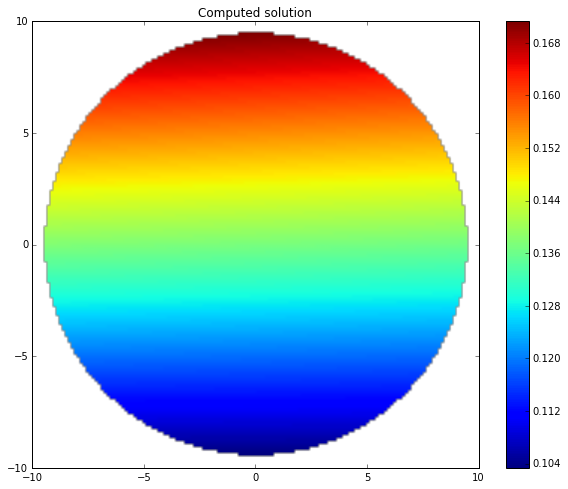
\includegraphics[width=10cm]{Imagenes/graficas/Situacion 1/Solucion ecuacion 1/2d.png}
\caption{Solución situacion 1}
\end{figure}

\begin{tcolorbox}
\begin{Verbatim}[commandchars=\\\{\}]
\PY{c+c1}{\PYZsh{}Import libraries}
\PY{k+kn}{import} \PY{n+nn}{bempp}\PY{n+nn}{.}\PY{n+nn}{api}
\PY{k+kn}{import} \PY{n+nn}{numpy} \PY{k}{as} \PY{n+nn}{np}
\PY{k+kn}{import} \PY{n+nn}{timeit}
\PY{n}{bempp}\PY{o}{.}\PY{n}{api}\PY{o}{.}\PY{n}{set\PYZus{}ipython\PYZus{}notebook\PYZus{}viewer}\PY{p}{(}\PY{p}{)}
        
\PY{c+c1}{\PYZsh{}Set quadrature options}
\PY{n}{bempp}\PY{o}{.}\PY{n}{api}\PY{o}{.}\PY{n}{global\PYZus{}parameters}\PY{o}{.}\PY{n}{quadrature}\PY{o}{.}\PY{n}{near}\PY{o}{.}\PY{n}{double\PYZus{}order} \PY{o}{=} \PY{l+m+mi}{2}
\PY{n}{bempp}\PY{o}{.}\PY{n}{api}\PY{o}{.}\PY{n}{global\PYZus{}parameters}\PY{o}{.}\PY{n}{quadrature}\PY{o}{.}\PY{n}{medium}\PY{o}{.}\PY{n}{double\PYZus{}order} \PY{o}{=} \PY{l+m+mi}{2}
\PY{n}{bempp}\PY{o}{.}\PY{n}{api}\PY{o}{.}\PY{n}{global\PYZus{}parameters}\PY{o}{.}\PY{n}{quadrature}\PY{o}{.}\PY{n}{far}\PY{o}{.}\PY{n}{double\PYZus{}order} \PY{o}{=} \PY{l+m+mi}{2}
\end{Verbatim}
\end{tcolorbox}

\begin{tcolorbox}
\begin{Verbatim}[commandchars=\\\{\}]
\PY{c+c1}{\PYZsh{}Define grid}
\PY{n}{grid\PYZus{}0} \PY{o}{=} \PY{n}{bempp}\PY{o}{.}\PY{n}{api}\PY{o}{.}\PY{n}{import\PYZus{}grid}\PY{p}{(}\PY{l+s+s2}{\PYZdq{}}\PY{l+s+s2}{BH21\PYZus{}a5\PYZus{}l10\PYZus{}E5550.msh}\PY{l+s+s2}{\PYZdq{}}\PY{p}{)}
        
\PY{c+c1}{\PYZsh{} Print out the number of elements}
\PY{n}{number\PYZus{}of\PYZus{}elements} \PY{o}{=} \PY{n}{grid\PYZus{}0}\PY{o}{.}\PY{n}{leaf\PYZus{}view}\PY{o}{.}\PY{n}{entity\PYZus{}count}\PY{p}{(}\PY{l+m+mi}{0}\PY{p}{)}
\PY{n+nb}{print}\PY{p}{(}\PY{l+s+s2}{\PYZdq{}}\PY{l+s+s2}{The grid has }\PY{l+s+si}{\PYZob{}0\PYZcb{}}\PY{l+s+s2}{ elements.}\PY{l+s+s2}{\PYZdq{}}\PY{o}{.}\PY{n}{format}\PY{p}{(}\PY{n}{number\PYZus{}of\PYZus{}elements}\PY{p}{)}\PY{p}{)}
        
\PY{c+c1}{\PYZsh{}Plot the grid}
grid\PYZus{}0.plot()
\end{Verbatim}
\end{tcolorbox}

\begin{tcolorbox}
\begin{Verbatim}[commandchars=\\\{\}]
 \PY{c+c1}{\PYZsh{}Problem data}
\PY{n}{omega} \PY{o}{=} \PY{l+m+mf}{2.}\PY{o}{*}\PY{n}{np}\PY{o}{.}\PY{n}{pi}\PY{o}{*}\PY{l+m+mf}{10.e9}
\PY{n}{e0} \PY{o}{=} \PY{l+m+mf}{8.854}\PY{o}{*}\PY{l+m+mf}{1e\PYZhy{}12}\PY{o}{*}\PY{l+m+mf}{1e\PYZhy{}18}
\PY{n}{mu0} \PY{o}{=} \PY{l+m+mf}{4.}\PY{o}{*}\PY{n}{np}\PY{o}{.}\PY{n}{pi}\PY{o}{*}\PY{l+m+mf}{1e\PYZhy{}7}\PY{o}{*}\PY{l+m+mf}{1e6}
\PY{n}{mue} \PY{o}{=} \PY{p}{(}\PY{l+m+mf}{1.}\PY{p}{)}\PY{o}{*}\PY{n}{mu0}
\PY{n}{ee} \PY{o}{=} \PY{p}{(}\PY{l+m+mf}{16.}\PY{p}{)}\PY{o}{*}\PY{n}{e0}
\PY{n}{mui} \PY{o}{=} \PY{p}{(}\PY{o}{\PYZhy{}}\PY{l+m+mf}{2.9214}\PY{o}{+}\PY{l+m+mf}{0.5895}\PY{n}{j}\PY{p}{)}\PY{o}{*}\PY{n}{mu0}
\PY{n}{ei} \PY{o}{=} \PY{p}{(}\PY{l+m+mf}{82629.2677}\PY{o}{\PYZhy{}}\PY{l+m+mf}{200138.2211}\PY{n}{j}\PY{p}{)}\PY{o}{*}\PY{n}{e0}
\PY{n}{k} \PY{o}{=} \PY{n}{omega}\PY{o}{*}\PY{n}{np}\PY{o}{.}\PY{n}{sqrt}\PY{p}{(}\PY{n}{e0}\PY{o}{*}\PY{n}{mu0}\PY{p}{)}
\PY{n}{lam} \PY{o}{=} \PY{l+m+mi}{2}\PY{o}{*}\PY{n}{np}\PY{o}{.}\PY{n}{pi}\PY{o}{/}\PY{n}{k}
\PY{n}{nm} \PY{o}{=} \PY{n}{np}\PY{o}{.}\PY{n}{sqrt}\PY{p}{(}\PY{p}{(}\PY{n}{ee}\PY{o}{*}\PY{n}{mue}\PY{p}{)}\PY{o}{/}\PY{p}{(}\PY{n}{e0}\PY{o}{*}\PY{n}{mu0}\PY{p}{)}\PY{p}{)}
\PY{n}{nc} \PY{o}{=} \PY{n}{np}\PY{o}{.}\PY{n}{sqrt}\PY{p}{(}\PY{p}{(}\PY{n}{ei}\PY{o}{*}\PY{n}{mui}\PY{p}{)}\PY{o}{/}\PY{p}{(}\PY{n}{e0}\PY{o}{*}\PY{n}{mu0}\PY{p}{)}\PY{p}{)}
\PY{n}{alfa\PYZus{}m} \PY{o}{=} \PY{n}{mue}\PY{o}{/}\PY{n}{mu0}
\PY{n}{alfa\PYZus{}c} \PY{o}{=} \PY{n}{mui}\PY{o}{/}\PY{n}{mue}
\PY{n}{antena} \PY{o}{=} \PY{n}{np}\PY{o}{.}\PY{n}{array}\PY{p}{(}\PY{p}{[}\PY{p}{[}\PY{l+m+mf}{1e4}\PY{p}{]}\PY{p}{,}\PY{p}{[}\PY{l+m+mf}{0.}\PY{p}{]}\PY{p}{,}\PY{p}{[}\PY{l+m+mf}{0.}\PY{p}{]}\PY{p}{]}\PY{p}{)}
\PY{n}{Amp} \PY{o}{=} \PY{l+m+mi}{1}
\PY{n+nb}{print}\PY{p}{(}\PY{l+s+s2}{\PYZdq{}}\PY{l+s+s2}{Numero de onda exterior:}\PY{l+s+s2}{\PYZdq{}}\PY{p}{,} \PY{n}{k}\PY{p}{)}
\PY{n+nb}{print}\PY{p}{(}\PY{l+s+s2}{\PYZdq{}}\PY{l+s+s2}{Indice de refraccion matriz:}\PY{l+s+s2}{\PYZdq{}}\PY{p}{,} \PY{n}{nm}\PY{p}{)}
\PY{n+nb}{print}\PY{p}{(}\PY{l+s+s2}{\PYZdq{}}\PY{l+s+s2}{Indice de refraccion conductor:}\PY{l+s+s2}{\PYZdq{}}\PY{p}{,} \PY{n}{nc}\PY{p}{)}
\PY{n+nb}{print}\PY{p}{(}\PY{l+s+s2}{\PYZdq{}}\PY{l+s+s2}{Numero de onda interior matriz:}\PY{l+s+s2}{\PYZdq{}}\PY{p}{,} \PY{n}{nm}\PY{o}{*}\PY{n}{k}\PY{p}{)}
\PY{n+nb}{print}\PY{p}{(}\PY{l+s+s2}{\PYZdq{}}\PY{l+s+s2}{Numero de onda interior conductor:}\PY{l+s+s2}{\PYZdq{}}\PY{p}{,} \PY{n}{nm}\PY{o}{*}\PY{n}{nc}\PY{o}{*}\PY{n}{k}\PY{p}{)}
\PY{n+nb}{print}\PY{p}{(}\PY{l+s+s2}{\PYZdq{}}\PY{l+s+s2}{Indice de transmision matriz:}\PY{l+s+s2}{\PYZdq{}}\PY{p}{,} \PY{n}{alfa\PYZus{}m}\PY{p}{)}
\PY{n+nb}{print}\PY{p}{(}\PY{l+s+s2}{\PYZdq{}}\PY{l+s+s2}{Indice de transmision conductor:}\PY{l+s+s2}{\PYZdq{}}\PY{p}{,} \PY{n}{alfa\PYZus{}c}\PY{p}{)}
\PY{n+nb}{print}\PY{p}{(}\PY{l+s+s2}{\PYZdq{}}\PY{l+s+s2}{Longitud de onda:}\PY{l+s+s2}{\PYZdq{}}\PY{p}{,} \PY{n}{lam}\PY{p}{,} \PY{l+s+s2}{\PYZdq{}}\PY{l+s+s2}{micras}\PY{l+s+s2}{\PYZdq{}}\PY{p}{)}
\end{Verbatim}
\end{tcolorbox}

\begin{tcolorbox}
\begin{Verbatim}[commandchars=\\\{\}]
\PY{c+c1}{\PYZsh{}Dirichlet and Neumann functions}
\PY{k}{def} \PY{n+nf}{dirichlet\PYZus{}fun}\PY{p}{(}\PY{n}{x}\PY{p}{,} \PY{n}{n}\PY{p}{,} \PY{n}{domain\PYZus{}index}\PY{p}{,} \PY{n}{result}\PY{p}{)}\PY{p}{:}
	\PY{n}{result}\PY{p}{[}\PY{l+m+mi}{0}\PY{p}{]} \PY{o}{=} \PY{n}{Amp} \PY{o}{*} \PY{n}{np}\PY{o}{.}\PY{n}{exp}\PY{p}{(}\PY{l+m+mi}{1}\PY{n}{j} \PY{o}{*} \PY{n}{k} \PY{o}{*} \PY{n}{x}\PY{p}{[}\PY{l+m+mi}{1}\PY{p}{]}\PY{p}{)}
\PY{k}{def} \PY{n+nf}{neumann\PYZus{}fun}\PY{p}{(}\PY{n}{x}\PY{p}{,} \PY{n}{n}\PY{p}{,} \PY{n}{domain\PYZus{}index}\PY{p}{,} \PY{n}{result}\PY{p}{)}\PY{p}{:}
	\PY{n}{result}\PY{p}{[}\PY{l+m+mi}{0}\PY{p}{]} \PY{o}{=} \PY{n}{Amp} \PY{o}{*} \PY{l+m+mi}{1}\PY{n}{j} \PY{o}{*} \PY{n}{k} \PY{o}{*} \PY{n}{n}\PY{p}{[}\PY{l+m+mi}{1}\PY{p}{]} \PY{o}{*} \PY{n}{np}\PY{o}{.}\PY{n}{exp}\PY{p}{(}\PY{l+m+mi}{1}\PY{n}{j} \PY{o}{*} \PY{n}{k} \PY{o}{*} \PY{n}{x}\PY{p}{[}\PY{l+m+mi}{1}\PY{p}{]}\PY{p}{)}
\end{Verbatim}
\end{tcolorbox}


\begin{tcolorbox}
\begin{Verbatim}[commandchars=\\\{\}]
\PY{c+c1}{\PYZsh{}Multitrace Operators}
\PY{n}{Ai\PYZus{}0} \PY{o}{=} \PY{n}{bempp}\PY{o}{.}\PY{n}{api}\PY{o}{.}\PY{n}{operators}\PY{o}{.}\PY{n}{boundary}\PY{o}{.}\PY{n}{helmholtz}\PY{o}{.}\PY{n}{multitrace\PYZus{}operator}\PY{p}{(}\PY{n}{grid\PYZus{}0}\PY{p}{,} 
	\PY{n}{nm} \PY{o}{*} \PY{n}{nc} \PY{o}{*} \PY{n}{k}\PY{p}{)}
\PY{n}{Ae\PYZus{}0} \PY{o}{=} \PY{n}{bempp}\PY{o}{.}\PY{n}{api}\PY{o}{.}\PY{n}{operators}\PY{o}{.}\PY{n}{boundary}\PY{o}{.}\PY{n}{helmholtz}\PY{o}{.}\PY{n}{multitrace\PYZus{}operator}\PY{p}{(}\PY{n}{grid\PYZus{}0}\PY{p}{,} 
	\PY{n}{nm} \PY{o}{*} \PY{n}{k}\PY{p}{)}
        
\PY{c+c1}{\PYZsh{}Multitrace Transmission}
\PY{n}{Ai\PYZus{}0}\PY{p}{[}\PY{l+m+mi}{0}\PY{p}{,}\PY{l+m+mi}{1}\PY{p}{]} \PY{o}{=} \PY{n}{Ai\PYZus{}0}\PY{p}{[}\PY{l+m+mi}{0}\PY{p}{,}\PY{l+m+mi}{1}\PY{p}{]}\PY{o}{*}\PY{n}{alfa\PYZus{}c}
\PY{n}{Ai\PYZus{}0}\PY{p}{[}\PY{l+m+mi}{1}\PY{p}{,}\PY{l+m+mi}{1}\PY{p}{]} \PY{o}{=} \PY{n}{Ai\PYZus{}0}\PY{p}{[}\PY{l+m+mi}{1}\PY{p}{,}\PY{l+m+mi}{1}\PY{p}{]}\PY{o}{*}\PY{n}{alfa\PYZus{}c}
        
\PY{c+c1}{\PYZsh{}Interior and exterior link up}
\PY{n}{op\PYZus{}0} \PY{o}{=} \PY{p}{(}\PY{n}{Ai\PYZus{}0} \PY{o}{+} \PY{n}{Ae\PYZus{}0}\PY{p}{)}
\end{Verbatim}
\end{tcolorbox}

\begin{tcolorbox}
\begin{Verbatim}[commandchars=\\\{\}]
\PY{c+c1}{\PYZsh{}Spaces}
\PY{n}{dirichlet\PYZus{}space\PYZus{}0} \PY{o}{=} \PY{n}{Ai\PYZus{}0}\PY{p}{[}\PY{l+m+mi}{0}\PY{p}{,}\PY{l+m+mi}{0}\PY{p}{]}\PY{o}{.}\PY{n}{domain}
\PY{n}{neumann\PYZus{}space\PYZus{}0} \PY{o}{=} \PY{n}{Ai\PYZus{}0}\PY{p}{[}\PY{l+m+mi}{0}\PY{p}{,}\PY{l+m+mi}{1}\PY{p}{]}\PY{o}{.}\PY{n}{domain}
\end{Verbatim}
\end{tcolorbox}

\begin{tcolorbox}
\begin{Verbatim}[commandchars=\\\{\}]
\PY{c+c1}{\PYZsh{}Identity}
\PY{n}{ident\PYZus{}0} \PY{o}{=} \PY{n}{bempp}\PY{o}{.}\PY{n}{api}\PY{o}{.}\PY{n}{operators}\PY{o}{.}\PY{n}{boundary}\PY{o}{.}\PY{n}{sparse}\PY{o}{.}\PY{n}{identity}\PY{p}{(}\PY{n}{neumann\PYZus{}space\PYZus{}0}\PY{p}{,} 
		\PY{n}{neumann\PYZus{}space\PYZus{}0}\PY{p}{,} \PY{n}{neumann\PYZus{}space\PYZus{}0}\PY{p}{)}
\end{Verbatim}
\end{tcolorbox}


\begin{tcolorbox}
\begin{Verbatim}[commandchars=\\\{\}]
\PY{c+c1}{\PYZsh{}Left hand side }
\PY{n}{blocked} \PY{o}{=} \PY{n}{bempp}\PY{o}{.}\PY{n}{api}\PY{o}{.}\PY{n}{BlockedOperator}\PY{p}{(}\PY{l+m+mi}{2}\PY{p}{,}\PY{l+m+mi}{2}\PY{p}{)}
\PY{n}{blocked}\PY{p}{[}\PY{l+m+mi}{0}\PY{p}{,}\PY{l+m+mi}{0}\PY{p}{]} \PY{o}{=} \PY{n}{op\PYZus{}0}\PY{p}{[}\PY{l+m+mi}{0}\PY{p}{,}\PY{l+m+mi}{0}\PY{p}{]}
\PY{n}{blocked}\PY{p}{[}\PY{l+m+mi}{0}\PY{p}{,}\PY{l+m+mi}{1}\PY{p}{]} \PY{o}{=} \PY{n}{op\PYZus{}0}\PY{p}{[}\PY{l+m+mi}{0}\PY{p}{,}\PY{l+m+mi}{1}\PY{p}{]}
\PY{n}{blocked}\PY{p}{[}\PY{l+m+mi}{1}\PY{p}{,}\PY{l+m+mi}{0}\PY{p}{]} \PY{o}{=} \PY{n}{op\PYZus{}0}\PY{p}{[}\PY{l+m+mi}{1}\PY{p}{,}\PY{l+m+mi}{0}\PY{p}{]}
\PY{n}{blocked}\PY{p}{[}\PY{l+m+mi}{1}\PY{p}{,}\PY{l+m+mi}{1}\PY{p}{]} \PY{o}{=} \PY{n}{op\PYZus{}0}\PY{p}{[}\PY{l+m+mi}{1}\PY{p}{,}\PY{l+m+mi}{1}\PY{p}{]}
\PY{n}{blocked}\PY{p}{[}\PY{l+m+mi}{1}\PY{p}{,}\PY{l+m+mi}{1}\PY{p}{]} \PY{o}{=} \PY{n}{blocked}\PY{p}{[}\PY{l+m+mi}{1}\PY{p}{,}\PY{l+m+mi}{1}\PY{p}{]} \PY{o}{+} \PY{l+m+mf}{0.5} \PY{o}{*} \PY{n}{ident\PYZus{}0} \PY{o}{*} \PY{p}{(}\PY{n}{alfa\PYZus{}c} \PY{o}{\PYZhy{}} \PY{l+m+mi}{1}\PY{p}{)}
        
\PY{c+c1}{\PYZsh{}Boundary conditions}
\PY{n}{dirichlet\PYZus{}grid\PYZus{}fun\PYZus{}0} \PY{o}{=} \PY{n}{bempp}\PY{o}{.}\PY{n}{api}\PY{o}{.}\PY{n}{GridFunction}\PY{p}{(}\PY{n}{dirichlet\PYZus{}space\PYZus{}0}\PY{p}{,} 
		\PY{n}{fun}\PY{o}{=}\PY{n}{dirichlet\PYZus{}fun}\PY{p}{)}
\PY{n}{neumann\PYZus{}grid\PYZus{}fun\PYZus{}0} \PY{o}{=} \PY{n}{bempp}\PY{o}{.}\PY{n}{api}\PY{o}{.}\PY{n}{GridFunction}\PY{p}{(}\PY{n}{neumann\PYZus{}space\PYZus{}0}\PY{p}{,} \PY{n}{fun}\PY{o}{=}\PY{n}{neumann\PYZus{}fun}\PY{p}{)}
\end{Verbatim}
\end{tcolorbox}

\begin{tcolorbox}
\begin{Verbatim}[commandchars=\\\{\}]
\PY{n}{start} \PY{o}{=} \PY{n}{timeit}\PY{o}{.}\PY{n}{default\PYZus{}timer}\PY{p}{(}\PY{p}{)}
\PY{c+c1}{\PYZsh{}Solving the matrix system}
\PY{n}{sol}\PY{p}{,} \PY{n}{info}\PY{p}{,} \PY{n}{it\PYZus{}count} \PY{o}{=} \PY{n}{bempp}\PY{o}{.}\PY{n}{api}\PY{o}{.}\PY{n}{linalg}\PY{o}{.}\PY{n}{gmres}\PY{p}{(}\PY{n}{blocked}\PY{p}{,} 
			\PY{p}{[}\PY{n}{dirichlet\PYZus{}grid\PYZus{}fun\PYZus{}0}\PY{p}{,} \PY{n}{neumann\PYZus{}grid\PYZus{}fun\PYZus{}0}\PY{p}{]}\PY{p}{,}
			\PY{n}{use\PYZus{}strong\PYZus{}form}\PY{o}{=}\PY{k+kc}{True}\PY{p}{,} \PY{n}{return\PYZus{}iteration\PYZus{}count}\PY{o}{=}\PY{k+kc}{True}\PY{p}{,} 
			\PY{n}{tol}\PY{o}{=}\PY{l+m+mf}{1e\PYZhy{}5}\PY{p}{,}\PY{n}{restart}\PY{o}{=}\PY{l+m+mi}{20}\PY{p}{,} \PY{n}{maxiter}\PY{o}{=}\PY{l+m+mi}{500000}\PY{p}{)}
\PY{n}{stop} \PY{o}{=} \PY{n}{timeit}\PY{o}{.}\PY{n}{default\PYZus{}timer}\PY{p}{(}\PY{p}{)}

\PY{c+c1}{\PYZsh{}Print iterations}
\PY{n+nb}{print}\PY{p}{(}\PY{l+s+s2}{\PYZdq{}}\PY{l+s+s2}{The linear system was solved in }\PY{l+s+si}{\PYZob{}0\PYZcb{}}\PY{l+s+s2}{ iterations}\PY{l+s+s2}{\PYZdq{}}\PY{o}{.}\PY{n}{format}\PY{p}{(}\PY{n}{it\PYZus{}count}\PY{p}{)}\PY{p}{)}
\PY{n+nb}{print}\PY{p}{(}\PY{l+s+s1}{\PYZsq{}}\PY{l+s+s1}{Time: }\PY{l+s+s1}{\PYZsq{}}\PY{p}{,} \PY{n}{stop} \PY{o}{\PYZhy{}} \PY{n}{start}\PY{p}{)}
\end{Verbatim}
\end{tcolorbox}


\begin{tcolorbox}
\begin{Verbatim}[commandchars=\\\{\}]
\PY{c+c1}{\PYZsh{}Divide the solution}
\PY{n}{solution\PYZus{}dirichl}\PY{p}{,} \PY{n}{solution\PYZus{}neumann} \PY{o}{=} \PY{n}{sol}
\PY{n+nb}{print}\PY{p}{(}\PY{n}{sol}\PY{p}{)}

\PY{c+c1}{\PYZsh{}Plot the solution}
\PY{n}{solution\PYZus{}neumann}\PY{o}{.}\PY{n}{plot}\PY{p}{(}\PY{p}{)}
\end{Verbatim}
\end{tcolorbox}


\begin{tcolorbox}
\begin{Verbatim}[commandchars=\\\{\}]
\PY{n}{Nx} \PY{o}{=} \PY{l+m+mi}{150}
\PY{n}{Ny} \PY{o}{=} \PY{l+m+mi}{150}
\PY{n}{di}\PY{o}{=}\PY{l+m+mi}{10}
\PY{n}{xmin}\PY{p}{,} \PY{n}{xmax}\PY{p}{,} \PY{n}{ymin}\PY{p}{,} \PY{n}{ymax} \PY{o}{=} \PY{p}{[}\PY{o}{\PYZhy{}}\PY{n}{di}\PY{p}{,}\PY{n}{di}\PY{p}{,}\PY{o}{\PYZhy{}}\PY{n}{di}\PY{p}{,}\PY{n}{di}\PY{p}{]}
\PY{n}{plot\PYZus{}grid} \PY{o}{=} \PY{n}{np}\PY{o}{.}\PY{n}{mgrid}\PY{p}{[}\PY{n}{xmin}\PY{p}{:}\PY{n}{xmax}\PY{p}{:}\PY{n}{Nx} \PY{o}{*} \PY{l+m+mi}{1}\PY{n}{j}\PY{p}{,} \PY{n}{ymin}\PY{p}{:}\PY{n}{ymax}\PY{p}{:}\PY{n}{Ny} \PY{o}{*} \PY{l+m+mi}{1}\PY{n}{j}\PY{p}{]}
\PY{n}{points} \PY{o}{=} \PY{n}{np}\PY{o}{.}\PY{n}{vstack}\PY{p}{(}\PY{p}{(}\PY{n}{plot\PYZus{}grid}\PY{p}{[}\PY{l+m+mi}{0}\PY{p}{]}\PY{o}{.}\PY{n}{ravel}\PY{p}{(}\PY{p}{)}\PY{p}{,}
			\PY{n}{plot\PYZus{}grid}\PY{p}{[}\PY{l+m+mi}{1}\PY{p}{]}\PY{o}{.}\PY{n}{ravel}\PY{p}{(}\PY{p}{)}\PY{p}{,}
            \PY{l+m+mi}{0}\PY{o}{*}\PY{n}{np}\PY{o}{.}\PY{n}{ones}\PY{p}{(}\PY{n}{plot\PYZus{}grid}\PY{p}{[}\PY{l+m+mi}{0}\PY{p}{]}\PY{o}{.}\PY{n}{size}\PY{p}{)}\PY{p}{)}\PY{p}{)}
\PY{n}{u\PYZus{}evaluated} \PY{o}{=} \PY{n}{np}\PY{o}{.}\PY{n}{zeros}\PY{p}{(}\PY{n}{points}\PY{o}{.}\PY{n}{shape}\PY{p}{[}\PY{l+m+mi}{1}\PY{p}{]}\PY{p}{,} \PY{n}{dtype}\PY{o}{=}\PY{n}{np}\PY{o}{.}\PY{n}{complex128}\PY{p}{)}
         
\PY{n}{x}\PY{p}{,} \PY{n}{y} \PY{o}{=} \PY{n}{points}\PY{p}{[}\PY{p}{:}\PY{l+m+mi}{2}\PY{p}{]}
\PY{n}{idx\PYZus{}ext} \PY{o}{=} \PY{n}{np}\PY{o}{.}\PY{n}{sqrt}\PY{p}{(}\PY{n}{x}\PY{o}{*}\PY{o}{*}\PY{l+m+mi}{2} \PY{o}{+} \PY{n}{y}\PY{o}{*}\PY{o}{*}\PY{l+m+mi}{2}\PY{p}{)} \PY{o}{\PYZgt{}} \PY{n}{di}
\PY{n}{idx\PYZus{}int} \PY{o}{=} \PY{n}{np}\PY{o}{.}\PY{n}{sqrt}\PY{p}{(}\PY{n}{x}\PY{o}{*}\PY{o}{*}\PY{l+m+mi}{2} \PY{o}{+} \PY{n}{y}\PY{o}{*}\PY{o}{*}\PY{l+m+mi}{2}\PY{p}{)} \PY{o}{\PYZlt{}}\PY{o}{=} \PY{n}{di}
         
\PY{n}{points\PYZus{}exterior} \PY{o}{=} \PY{n}{points}\PY{p}{[}\PY{p}{:}\PY{p}{,} \PY{n}{idx\PYZus{}ext}\PY{p}{]}
\PY{n}{points\PYZus{}interior} \PY{o}{=} \PY{n}{points}\PY{p}{[}\PY{p}{:}\PY{p}{,} \PY{n}{idx\PYZus{}int}\PY{p}{]}
\end{Verbatim}
\end{tcolorbox}


\begin{tcolorbox}
\begin{Verbatim}[commandchars=\\\{\}]
\PY{n}{slp\PYZus{}pot\PYZus{}int} \PY{o}{=} \PY{n}{bempp}\PY{o}{.}\PY{n}{api}\PY{o}{.}\PY{n}{operators}\PY{o}{.}\PY{n}{potential}\PY{o}{.}\PY{n}{helmholtz}\PY{o}{.}\PY{n}{single\PYZus{}layer}\PY{p}{(}
	\PY{n}{dirichlet\PYZus{}space\PYZus{}0}\PY{p}{,} \PY{n}{points\PYZus{}interior}\PY{p}{,} \PY{n}{nm} \PY{o}{*} \PY{n}{k}\PY{p}{)}
\PY{n}{slp\PYZus{}pot\PYZus{}ext} \PY{o}{=} \PY{n}{bempp}\PY{o}{.}\PY{n}{api}\PY{o}{.}\PY{n}{operators}\PY{o}{.}\PY{n}{potential}\PY{o}{.}\PY{n}{helmholtz}\PY{o}{.}\PY{n}{single\PYZus{}layer}\PY{p}{(}
	\PY{n}{dirichlet\PYZus{}space\PYZus{}0}\PY{p}{,} \PY{n}{points\PYZus{}exterior}\PY{p}{,} \PY{n}{k}\PY{p}{)}
\PY{n}{dlp\PYZus{}pot\PYZus{}int} \PY{o}{=} \PY{n}{bempp}\PY{o}{.}\PY{n}{api}\PY{o}{.}\PY{n}{operators}\PY{o}{.}\PY{n}{potential}\PY{o}{.}\PY{n}{helmholtz}\PY{o}{.}\PY{n}{double\PYZus{}layer}\PY{p}{(}
	\PY{n}{dirichlet\PYZus{}space\PYZus{}0}\PY{p}{,} \PY{n}{points\PYZus{}interior}\PY{p}{,} \PY{n}{nm} \PY{o}{*} \PY{n}{k}\PY{p}{)}
\PY{n}{dlp\PYZus{}pot\PYZus{}ext} \PY{o}{=} \PY{n}{bempp}\PY{o}{.}\PY{n}{api}\PY{o}{.}\PY{n}{operators}\PY{o}{.}\PY{n}{potential}\PY{o}{.}\PY{n}{helmholtz}\PY{o}{.}\PY{n}{double\PYZus{}layer}\PY{p}{(}
	\PY{n}{dirichlet\PYZus{}space\PYZus{}0}\PY{p}{,} \PY{n}{points\PYZus{}exterior}\PY{p}{,} \PY{n}{k}\PY{p}{)}
         
\PY{n}{total\PYZus{}field\PYZus{}int} \PY{o}{=} \PY{p}{(}\PY{n}{slp\PYZus{}pot\PYZus{}int} \PY{o}{*} \PY{n}{solution\PYZus{}neumann} 
			\PY{o}{\PYZhy{}} \PY{n}{dlp\PYZus{}pot\PYZus{}int} \PY{o}{*} \PY{n}{solution\PYZus{}dirichl}\PY{p}{)}\PY{o}{.}\PY{n}{ravel}\PY{p}{(}\PY{p}{)}
\PY{n}{total\PYZus{}field\PYZus{}ext} \PY{o}{=} \PY{p}{(}\PY{n}{dlp\PYZus{}pot\PYZus{}ext} \PY{o}{*} \PY{n}{solution\PYZus{}dirichl} 
			\PY{o}{\PYZhy{}} \PY{n}{slp\PYZus{}pot\PYZus{}ext} \PY{o}{*} \PY{n}{solution\PYZus{}neumann}\PY{p}{)}\PY{o}{.}\PY{n}{ravel}\PY{p}{(}\PY{p}{)} \PYZbs{}
             \PY{o}{+} \PY{n}{np}\PY{o}{.}\PY{n}{exp}\PY{p}{(}\PY{l+m+mi}{1}\PY{n}{j} \PY{o}{*} \PY{n}{k} \PY{o}{*} \PY{n}{points\PYZus{}exterior}\PY{p}{[}\PY{l+m+mi}{0}\PY{p}{]}\PY{p}{)}
         
\PY{n}{total\PYZus{}field} \PY{o}{=} \PY{n}{np}\PY{o}{.}\PY{n}{zeros}\PY{p}{(}\PY{n}{points}\PY{o}{.}\PY{n}{shape}\PY{p}{[}\PY{l+m+mi}{1}\PY{p}{]}\PY{p}{,} \PY{n}{dtype}\PY{o}{=}\PY{l+s+s1}{\PYZsq{}}\PY{l+s+s1}{complex128}\PY{l+s+s1}{\PYZsq{}}\PY{p}{)}
\PY{n}{total\PYZus{}field}\PY{p}{[}\PY{n}{idx\PYZus{}ext}\PY{p}{]} \PY{o}{=} \PY{n}{total\PYZus{}field\PYZus{}ext}
\PY{n}{total\PYZus{}field}\PY{p}{[}\PY{n}{idx\PYZus{}int}\PY{p}{]} \PY{o}{=} \PY{n}{total\PYZus{}field\PYZus{}int}
\PY{n}{total\PYZus{}field} \PY{o}{=} \PY{n}{total\PYZus{}field}\PY{o}{.}\PY{n}{reshape}\PY{p}{(}\PY{p}{[}\PY{n}{Nx}\PY{p}{,} \PY{n}{Ny}\PY{p}{]}\PY{p}{)}
\end{Verbatim}
\end{tcolorbox}

\begin{tcolorbox}
\begin{Verbatim}[commandchars=\\\{\}]
\PY{o}{\PYZpc{}}\PY{k}{matplotlib} inline
\PY{k+kn}{from} \PY{n+nn}{matplotlib} \PY{k}{import} \PY{n}{pylab} \PY{k}{as} \PY{n}{plt}
\PY{n}{radius} \PY{o}{=} \PY{n}{np}\PY{o}{.}\PY{n}{sqrt}\PY{p}{(}\PY{n}{plot\PYZus{}grid}\PY{p}{[}\PY{l+m+mi}{0}\PY{p}{]}\PY{o}{*}\PY{o}{*}\PY{l+m+mi}{2} \PY{o}{+} \PY{n}{plot\PYZus{}grid}\PY{p}{[}\PY{l+m+mi}{1}\PY{p}{]}\PY{o}{*}\PY{o}{*}\PY{l+m+mi}{2}\PY{p}{)}
\PY{n}{total\PYZus{}field}\PY{p}{[}\PY{n}{radius}\PY{o}{\PYZgt{}}\PY{n}{di}\PY{p}{]} \PY{o}{=} \PY{n}{np}\PY{o}{.}\PY{n}{nan}
\PY{n}{fig} \PY{o}{=} \PY{n}{plt}\PY{o}{.}\PY{n}{figure}\PY{p}{(}\PY{n}{figsize}\PY{o}{=}\PY{p}{(}\PY{l+m+mi}{10}\PY{p}{,} \PY{l+m+mi}{10}\PY{p}{)}\PY{p}{)}
\PY{n}{plt}\PY{o}{.}\PY{n}{imshow}\PY{p}{(}\PY{n}{np}\PY{o}{.}\PY{n}{real}\PY{p}{(}\PY{n}{total\PYZus{}field}\PY{o}{.}\PY{n}{T}\PY{p}{)}\PY{p}{,} \PY{n}{extent}\PY{o}{=}\PY{p}{[}\PY{o}{\PYZhy{}}\PY{n}{di}\PY{p}{,}\PY{n}{di}\PY{p}{,}\PY{o}{\PYZhy{}}\PY{n}{di}\PY{p}{,}\PY{n}{di}\PY{p}{]}\PY{p}{)}
\PY{n}{plt}\PY{o}{.}\PY{n}{xlabel}\PY{p}{(}\PY{l+s+s1}{\PYZsq{}}\PY{l+s+s1}{x}\PY{l+s+s1}{\PYZsq{}}\PY{p}{)}
\PY{n}{plt}\PY{o}{.}\PY{n}{ylabel}\PY{p}{(}\PY{l+s+s1}{\PYZsq{}}\PY{l+s+s1}{y}\PY{l+s+s1}{\PYZsq{}}\PY{p}{)}
\PY{n}{plt}\PY{o}{.}\PY{n}{colorbar}\PY{p}{(}\PY{p}{)}
\end{Verbatim}
\end{tcolorbox}
